\documentclass[a4paper,14pt]{article}
\usepackage{blindtext}
\usepackage[T2A]{fontenc}
\usepackage[utf8]{inputenc}
\usepackage[english,russian]{babel}
\usepackage{listings}
\usepackage{geometry}
\usepackage{amssymb}
\usepackage{amsmath}
\usepackage[14pt]{extsizes}
\geometry{left=3cm}
\geometry{right=1.5cm}
\geometry{top=2cm}
\geometry{bottom=2cm}
\pagestyle{plain}
\usepackage{pgfplots}
\usepackage{filecontents}
\usepackage{graphicx}
\usepackage{indentfirst}
\DeclareGraphicsExtensions{.png}
\graphicspath{{images/}}
\usetikzlibrary{datavisualization}
\usetikzlibrary{datavisualization.formats.functions}
\usepackage{tabularx}
\pgfplotsset{width=7 cm}
\usepackage{xcolor}
%\renewcommand{\rmdefault}{ftm}
%\usepackage{mathptmx}
\usepackage{setspace}
% \usepackage{minted}

%\полуторный интервал
\onehalfspacing
\frenchspacing

\usepackage{tocloft}
\frenchspacing
\setcounter{page}{2}
\usepackage{multirow}
\usepackage{float}
\usepackage{multirow}

\renewcommand{\cftsecdotsep}{\cftdot}
\renewcommand{\cftsecleader}{\cftdotfill{\cftsecdotsep}}
\renewcommand{\cftsubsecleader}{\cftdotfill{\cftsecdotsep}}
\renewcommand{\cftsubsubsecleader}{\cftdotfill{\cftsecdotsep}}

%\renewcommand\cftchapdotsep{\cftdot}
%\renewcommand\cftsecdotsep{\cftdot}
%\renewcommand{\cftchapleader}{\cftdotfill{\cftchapdotsep}}

% Для измененных титулов глав:
% % подключаем нужные пакеты
%\definecolor{gray75}{gray}{0.75} % определяем цвет
%\newcommand{\hsp}{\hspace{20pt}} % длина линии в 20pt
% titleformat определяет стиль
%\titleformat{\chapter}[hang]{\Huge\bfseries}{\thechapter\hsp\textcolor{black}{|}\hsp}{0pt}{\Huge\bfseries}
%\usepackage{titlesec, blindtext, color}
%\titleformat{\chapter}[hang]{\Huge\bfseries}{\thechapter\hsp\textcolor{black}{|}\hsp}{0pt}{\Huge\bfseries}

\lstset{ %
extendedchars=\true,
inputencoding=utf8,
morekeywords={include, printf},
texcl=\true,
breaklines=\true,
escapeend=\end{russian},
escapechar=\%,
keepspaces=\true,
language=python,                 % выбор языка для подсветки
basicstyle=\small\sffamily, % размер и начертание шрифта для подсветки кода
numbers=left,               % где поставить нумерацию строк (слева\справа)
numberstyle=\tiny,           % размер шрифта для номеров строк
stepnumber=1,                   % размер шага между двумя номерами строк
numbersep=5pt,                % как далеко отстоят номера строк от подсвечиваемого кода
showspaces=\true,            % показывать или нет пробелы специальными отступами
showstringspaces=\true,      % показывать или нет пробелы в строках
showtabs=false,             % показывать или нет табуляцию в строках
frame=single,              % рисовать рамку вокруг кода
tabsize=4,                 % размер табуляции по умолчанию равен 2 пробелам
captionpos=t,              % позиция заголовка вверху [t] или внизу [b]
breaklines=true,           % автоматически переносить строки (да\нет)
breakatwhitespace=false, % переносить строки только если есть пробел
escapeinside={\#*}{*)}   % если нужно добавить комментарии в коде
}



\begin{document}
\pgfplotsset{compat=1.17}

\begin{titlepage}

    \begin{table}
        \centering
        \footnotesize
        \begin{tabular}{cc}
            \multirow{8}{*}{
\includegraphics[scale=0.35]{bmstu.jpg}}
            & \\
            & \\
            & \textbf{Министерство науки и высшего образования Российской Федерации} \\
            & \textbf{Федеральное государственное бюджетное образовательное учреждение} \\
            & \textbf{высшего образования} \\
            & \textbf{<<Московский государственный технический} \\
            & \textbf{университет имени Н.Э. Баумана>>} \\
            & \textbf{(МГТУ им. Н.Э. Баумана)} \\
        \end{tabular}
    \end{table}

    \vspace{-2.5cm}

    \begin{flushleft}
        \rule[-1cm]{\textwidth}{3pt}
        \rule{\textwidth}{1pt}
    \end{flushleft}

    \begin{flushleft}
		ФАКУЛЬТЕТ Информатика и системы управления 
	\end{flushleft}
        КАФЕДРА Программное обеспечение ЭВМ и информационные технологии

    \vspace{3cm}

    \begin{center}
		\textbf{Лабораторная работа № 5} \\
		\textbf{Дисциплина: <<Моделирование>>}
        \vspace{0.5cm}
	\end{center}

	\begin{center}
		\textbf{Тема: <<Исследование математической модели на основе технологии вычислительного эксперимента>>}
        \vspace{0.5cm}
    \end{center}

    \vspace{2cm}

	\begin{flushleft}
        \begin{tabular}{ll}
            \textbf{Студент} & Овчинникова А. П. \\
            \textbf{Группа} & ИУ7-65Б \\
            \textbf{Оценка (баллы)} & \\
            \textbf{Преподаватель} & Градов В.М.   \\
        \end{tabular}
    \end{flushleft}

    \vspace{2cm}

   \begin{center}
        Москва, 2020 г.
    \end{center}

\end{titlepage}

\setcounter{page}{2}

\subsection*{Цель работы}

Целью данной работы является получение навыков проведения исследований 
компьютерной математической модели, построенной на квазилинейном
 уравнении параболического типа. Исследование проводится  
 с помощью программы, созданной   в лабораторной работе №4. 

\subsection*{Исходные данные}

1. Значения параметров для отладки (все размерности согласованы).

\begin{table}[!h]
	\caption{\label{tab.canonsummary} Значения параматров.}
	\begin{center}
	\begin{tabular}{|c c|}
	\hline
	$k(T) = $ & $a_1 (b_1 + c_1 T^{m_1})$ Вт/см К \\
	$c(T) = $ & $a_2 + b_2 T^{m_2} - \frac{c_2}{T^2} $ Дж/см$^3$ К \\
	$a_1 = $ & 0.0134 \\
	$b_1 = $ & 1 \\
	$c_1 = $ & $4.35 \cdot 10^{-4} $ \\
	$m_1 = $ & 1 \\
	$a_2 = $ & 2.049 \\
	$b_2 = $ & $0.563 \cdot 10^{-3}$ \\
	$c_2 = $ & $0.528 \cdot 10^{5}$ \\
	$m_2 =$ & 1 \\
	$\alpha (x) =$ & $\frac{c}{x-d}$ \\
	$\alpha_0 =$ & 0.05 Вт/см$^2$ К \\
	$\alpha_N =$ & 0.01 Вт/см$^2$ К \\
	$l =$ & 10 см \\
	$T_0 =$ & 300 К \\
	$R =$ & 0.5 см \\
	\hline
	\end{tabular}
	\end{center}
	\end{table}

2. Поток тепла $F(t)$ при $x = 0$:

\begin{equation}
	F(t) = \frac{F_{max}}{t_{max}} t e^{- (t/t_{max} - 1)},
\end{equation}

где $F_{max}, t_{max}$ -- амплитуда импульса потока и время её достижения (Вт/см$^2$ и с).

\subsection*{Задание}

1. Провести исследование по выбору оптимальных шагов по времени $\tau$
и пространству $h$. Шаги должны быть максимально большими при сохранении устойчивости разностной схемы и заданной точности расчета.

Рассмотреть влияние на получаемые результаты амплитуды импульса $F_{max}$
и времени $t_{max}$ (определяют крутизну фронтов и длительность импульса). 

Точность расчета можно оценить разными способами.

\begin{itemize}
	\item Уменьшая шаги и наблюдая сходимость решений, как это делалось в лаб. работе №1. 
	\item Проверяя, соблюдается ли при выбранных $\tau, h$ баланс мощности после выхода на стационарное распределение температуры (в установившемся режиме), реализующееся при
	$F(t) = const$, т.е. в этом режиме  должно выполняться условие: подводимая мощность  равна отводимой. Имеем
	\begin{equation}
		\pi R^2 (F_0 - F_N) = 2 \pi R \iint\limits_0^l \alpha[T(x, t_M) - T_0] dx,
	\end{equation}

	окончательно

	\begin{equation}
		\left| \frac{F_0 - F_N}{ \frac{2}{R} \iint\limits_0^l \alpha[T(x, t_M) - T_0] dx } - 1 \right| \leq \varepsilon.
	\end{equation}

	Задать точность $\varepsilon$ примерно $10^{-2}$. Здесь
	$t_M$ -- время выхода на стационарный режим, т.е. когда температура перестает меняться с заданной точностью (см. лаб. работу №4).
\end{itemize}

Замечание. Варьируя параметры задачи, следует иметь ввиду, что решения, в которых температура превышает значения примерно 2000К, физического смысла не имеют и практического интереса не представляют.

2. График зависимости температуры $T(0, t)$ при 3-4 значениях параметров
$a_2$ и/или $b_2$ теплоемкости.

3. График зависимости температуры $T(0, t)$ (т.е. при $x = 0$ 
в частотном режиме теплового нагружения. Импульсы следуют один за другим с заданной частотой $\nu$
(частота определяется количеством импульсов в 1 секунду). 

Показать, что при большом количестве импульсов температурное поле начинает в точности воспроизводиться от импульса к импульсу.  
Продемонстрировать, как по мере роста частоты импульсов размах колебаний температуры уменьшается (вплоть до нуля), т.е. реализуется квазистационарный режим, при котором в торец поступает постоянный поток
$F_c = \nu \int \limits_0^{t_u} F(t) dt$. Здесь
$t_u$ -- длительность импульса, определяемая как момент времени, когда
$\frac{F_{t_u}}{F_{max}} \approx 0.05$.
Если взять прямоугольные импульсы длительностью $t_u$ , т.е.
$F(t) = const = F_0$, то $F_c = \nu F_0 t_u$.

Справка. Полученное температурное поле должно совпасть с результатом расчета
$T(x)$ по программе лаб. работы №3 при $F_0 = F_c$, разумеется при всех одинаковых параметрах модели, в частности, вместо
$k(T)$ надо использовать $k(x)$ из лаб. работы №3.


\subsection*{Результаты работы}

\subsubsection*{Задание 1}

С помощью (3) проанализируем подводимую и отводимую мощность
на разных шагах $\tau, h$. Возьмем $\varepsilon = 10^{-2}$.
Так как (2) не зависит от $\tau$, то баланс мощности
не зависит от $\tau$. Рассмотрим отдельно $h$.
Возьмем $h = 0.4, 0.3, 0.2, 0.1, 0.01, 0.001$.

В таблице 2 представлены результаты выполнения неравенства (3) в зависимости
от выбранных значений $h$.


\begin{table}[!h]
	\caption{Выполнение неравенства 2.}
	\begin{center}
	\begin{tabular}{| c | c |}
	\hline
	$h$ & Соблюдается ли баланс мощности \\
	\hline

	0.4 & нет \\
	0.3 & да \\
	0.2 & да \\
	0.1 & да \\
	0.01 & да \\
	0.001 & да \\

	\hline
	\end{tabular}
	\end{center}
\end{table}

Будем проводить измерения при $F_{max} = 50$.

Пусть $t_{max} = 20$. рассмотрим результаты работы программы
при различных значениях шага  $h$ и $\tau = 2$ (рисунок \ref{fig:202}). Аналогично на рисунках
\ref{fig:201}-\ref{fig:20001} представлены результаты работы программы при $\tau = 1, \tau = 0.1, \tau = 0.05, \tau = 0.01$
соответственно.  На рисунках \ref{fig:202}-\ref{fig:20001}  в первой строке представлены значения $h$.

\newpage
\begin{figure}[!h]
	\center{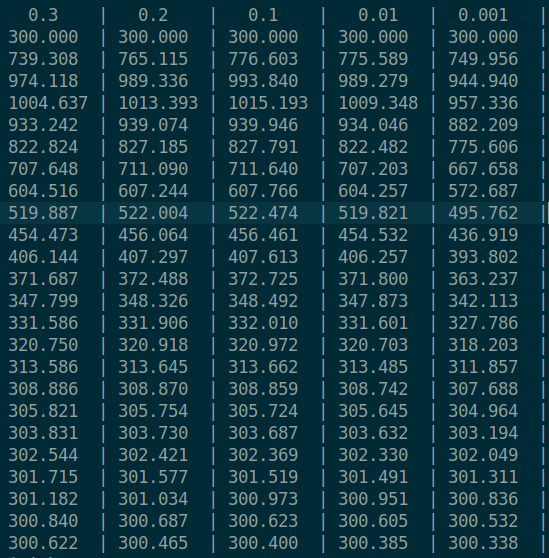
\includegraphics[width=13cm]{tau2}}
	\caption{$t_{max} = 20, \tau = 2$.}
	\label{fig:202}
\end{figure}

\newpage
\begin{figure}[!h]
	\center{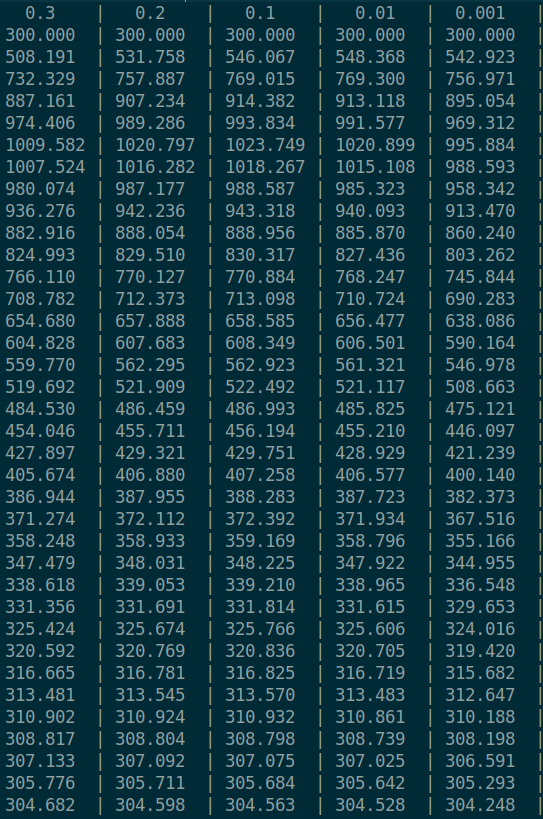
\includegraphics[width=13cm]{tau1}}
	\caption{$t_{max} = 20, \tau = 1$.}
	\label{fig:201}
\end{figure}
\newpage
\begin{figure}[!h]
	\center{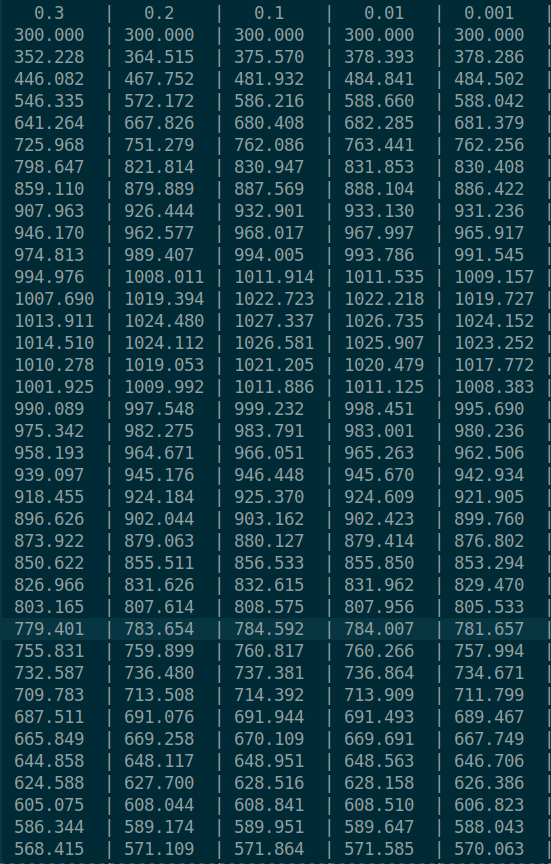
\includegraphics[width=13cm]{tau01}}
	\caption{$t_{max} = 20, \tau = 0.1$.}
	\label{fig:2001}
\end{figure}
\newpage
\begin{figure}[!h]
	\center{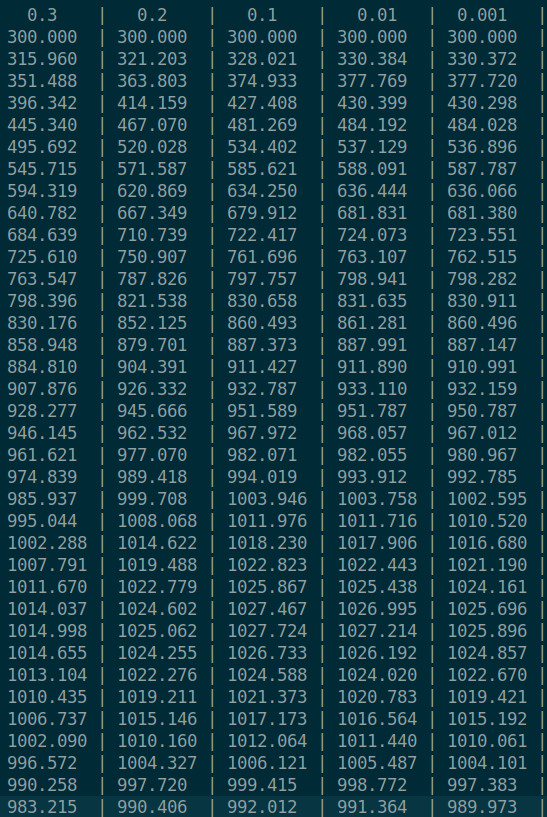
\includegraphics[width=13cm]{tau005}}
	\caption{$t_{max} = 20, \tau = 0.05$.}
	\label{fig:20005}
\end{figure}

\newpage
\begin{figure}[!h]
	\center{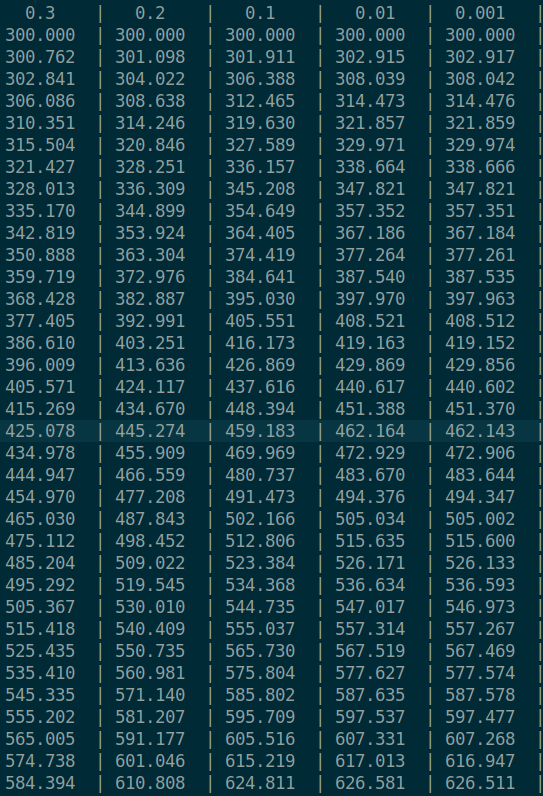
\includegraphics[width=13cm]{tau001}}
	\caption{$t_{max} = 20, \tau = 0.01$.}
	\label{fig:20001}
\end{figure}

Таким образом, при $F_{max} = 50, t_{max} = 20$ оптимальными значениями
шагов по времени и пространству являются $h = 0.01, \tau = 0.01$.

Пусть $t_{max} = 60$. Рассмотрим результаты работы программы
при различных значениях шага  $h$ и $\tau = 2$ (рисунок \ref{fig:602}). Аналогично на рисунках
\ref{fig:602}-\ref{fig:60001} представлены результаты работы программы при $\tau = 1, \tau = 0.1, \tau = 0.05, \tau = 0.01$
соответственно.  На рисунках \ref{fig:601}-\ref{fig:60001} в первой строке представлены значения $h$.

\newpage
\begin{figure}[!h]
	\center{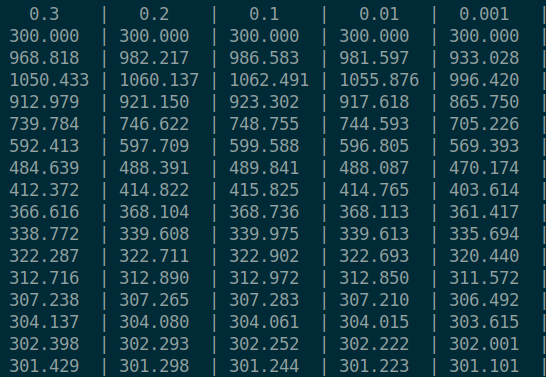
\includegraphics[width=13cm]{tau2tmax60}}
	\caption{$t_{max} = 60, \tau = 2$.}
	\label{fig:602}
\end{figure}

\newpage
\begin{figure}[!h]
	\center{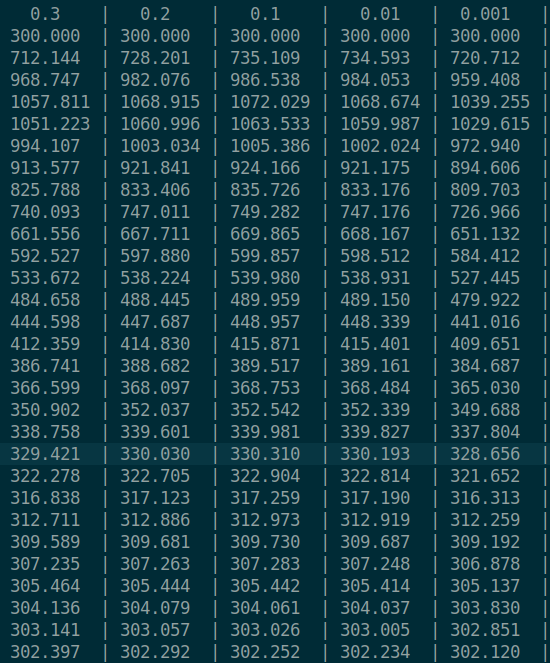
\includegraphics[width=13cm]{tau1tmax60}}
	\caption{$t_{max} = 60, \tau = 1$.}
	\label{fig:601}
\end{figure}

\newpage
\begin{figure}[!h]
	\center{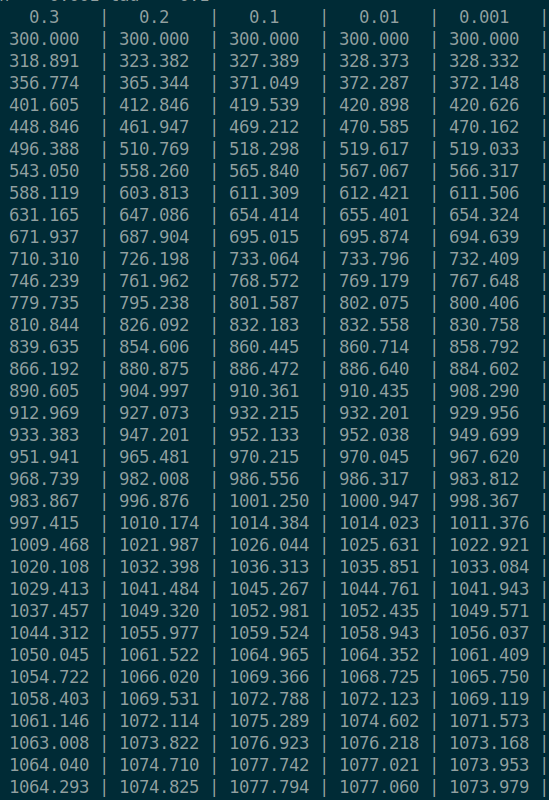
\includegraphics[width=13cm]{tau01tmax60}}
	\caption{$t_{max} = 60, \tau = 0.1$.}
	\label{fig:6001}
\end{figure}

\newpage
\begin{figure}[!h]
	\center{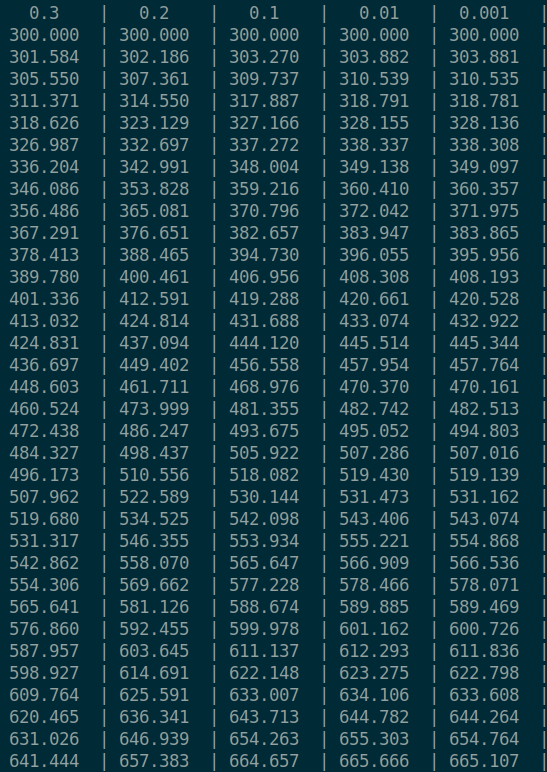
\includegraphics[width=13cm]{tau005tmax60}}
	\caption{$t_{max} = 60, \tau = 0.05$.}
	\label{fig:60005}
\end{figure}

\newpage
\begin{figure}[!h]
	\center{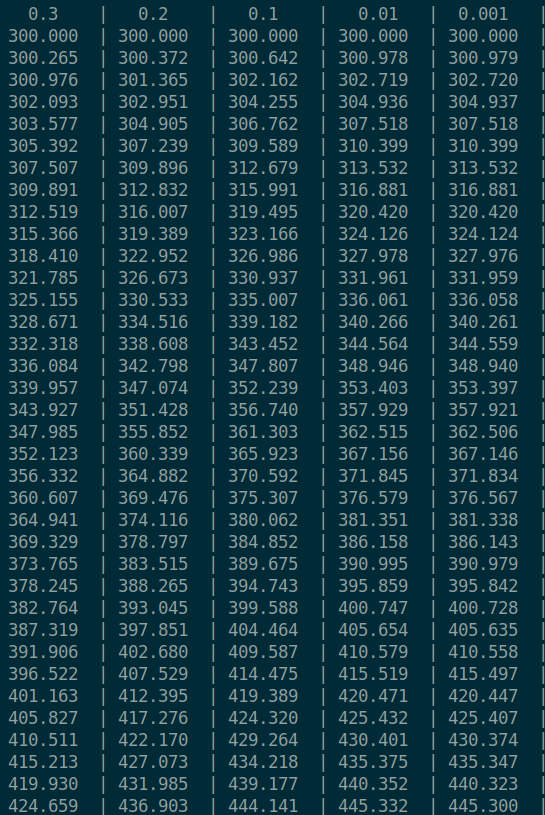
\includegraphics[width=13cm]{tau001tmax60}}
	\caption{$t_{max} = 60, \tau = 0.01$.}
	\label{fig:60001}
\end{figure}

Таким образом, при $t_{max} = 60, F_{max} = 50$, оптимальными
значениями шагов являются $h = 0.01, \tau = 0.01$.

Пусть $t_{max} = 100$. рассмотрим результаты работы программы
при различных значениях шага  $h$ и $\tau = 2$ (рисунок \ref{fig:1002}). Аналогично на рисунках
\ref{fig:1002}-\ref{fig:100001} представлены результаты работы программы при $\tau = 1, \tau = 0.1, \tau = 0.05, \tau = 0.01$
соответственно.  На рисунках \ref{fig:1002}-\ref{fig:100001} в первой строке представлены значения $h$.

\begin{figure}[!h]
	\center{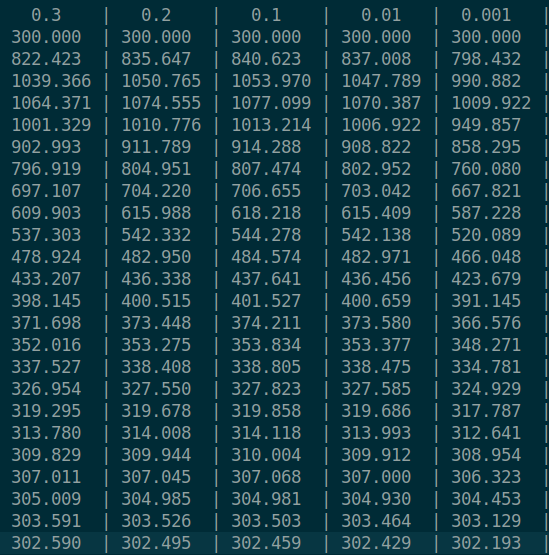
\includegraphics[width=13cm]{tau2tmax100}}
	\caption{$t_{max} = 100, \tau = 2$.}
	\label{fig:1002}
\end{figure}
\newpage
\begin{figure}[!h]
	\center{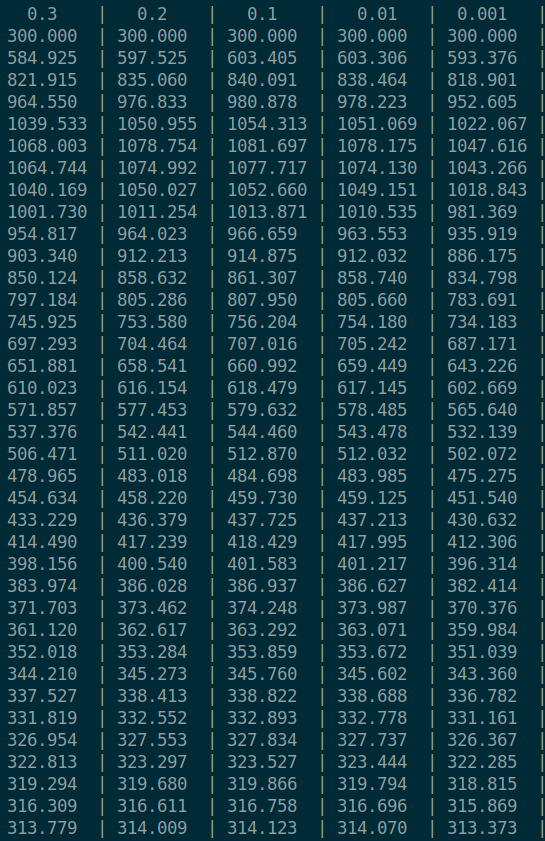
\includegraphics[width=13cm]{tau1tmax100}}
	\caption{$t_{max} = 100, \tau = 1$.}
	\label{fig:1001}
\end{figure}
\newpage
\begin{figure}[!h]
	\center{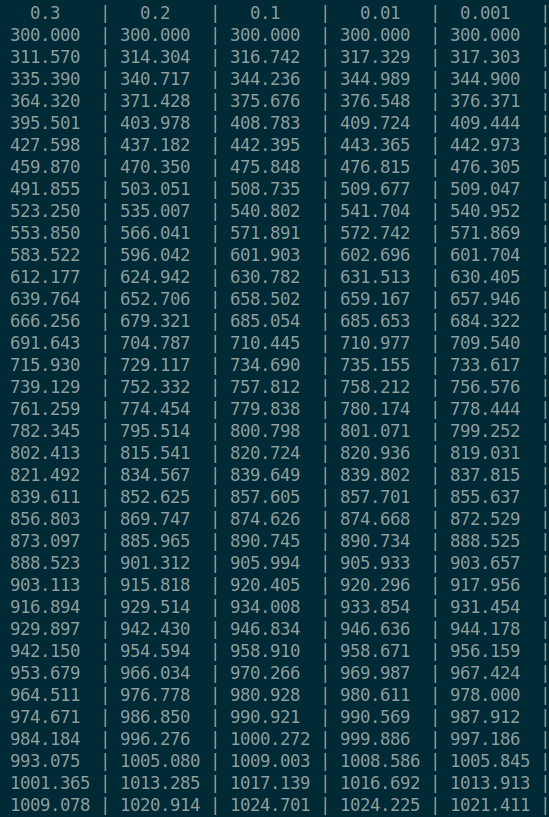
\includegraphics[width=13cm]{tau01tmax100}}
	\caption{$t_{max} = 100, \tau = 0.1$.}
	\label{fig:10001}
\end{figure}
\newpage
\begin{figure}[!h]
	\center{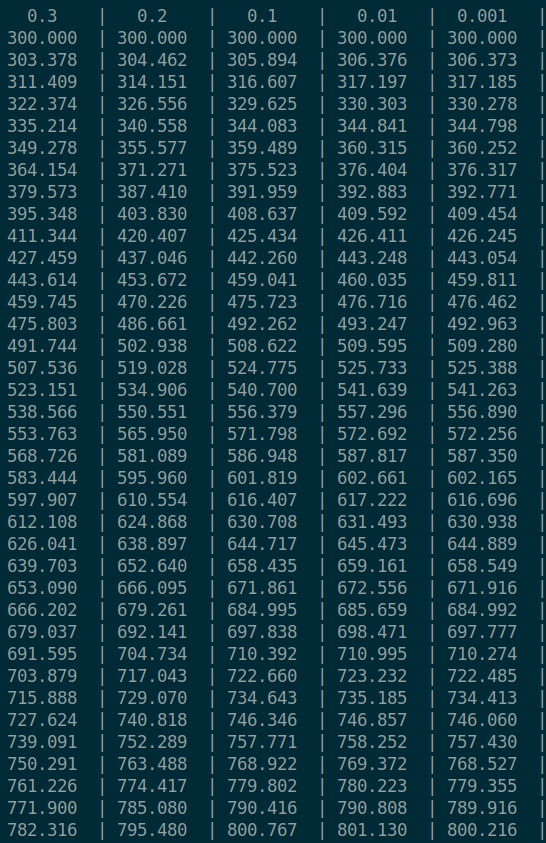
\includegraphics[width=13cm]{tau005tmax100}}
	\caption{$t_{max} = 100, \tau = 0.05$.}
	\label{fig:100005}
\end{figure}
\newpage
\begin{figure}[!h]
	\center{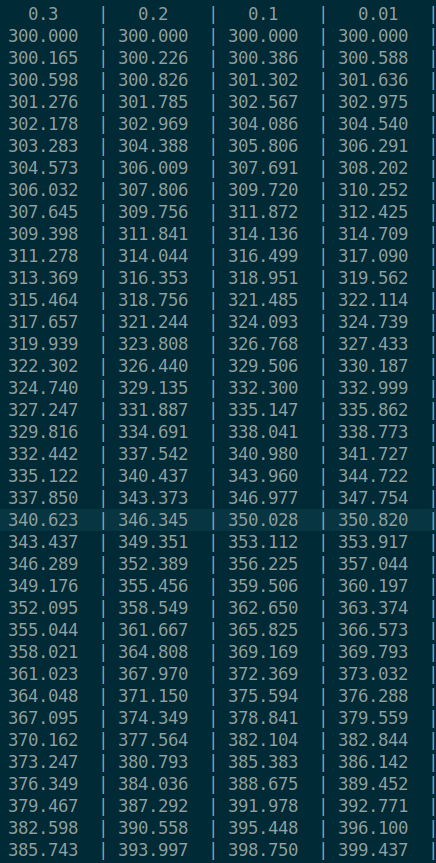
\includegraphics[width=12cm]{tau001tmax100}}
	\caption{$t_{max} = 100, \tau = 0.01$.}
	\label{fig:100001}
\end{figure}

Таким образом, при $t_{max} = 100, F_{max} = 50$, оптимальными
значениями шагов являются $h = 0.01, \tau = 0.1$.

Пусть $t_{max} = 140$. Рассмотрим результаты работы программы
при различных значениях шага  $h$ и $\tau = $ (рисунок \ref{fig:1402}). Аналогично на рисунках
\ref{fig:1401}-\ref{fig:140001} представлены результаты работы программы при $\tau = 1, \tau = 0.1, \tau = 0.05, \tau = 0.01$
соответственно.  На рисунках \ref{fig:1402}-\ref{fig:140001} в первой строке представлены значения $h$.
\begin{figure}[!h]
	\center{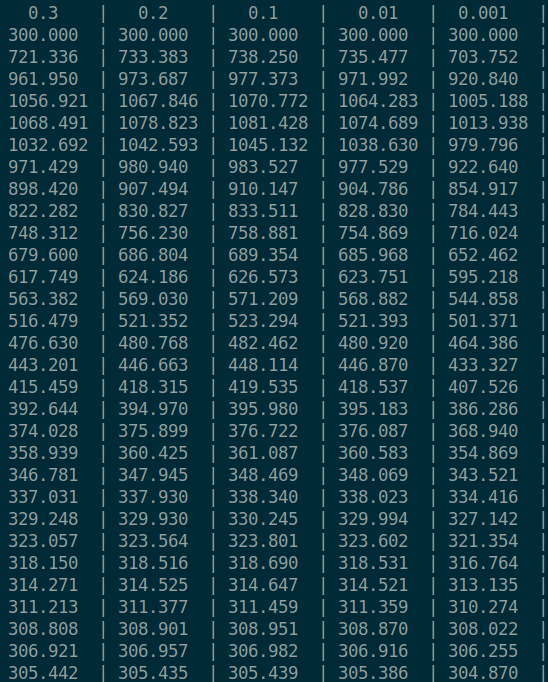
\includegraphics[width=12cm]{tau2tmax140}}
	\caption{$t_{max} = 140, \tau = 2$.}
	\label{fig:1402}
\end{figure}
\newpage
\begin{figure}[!h]
	\center{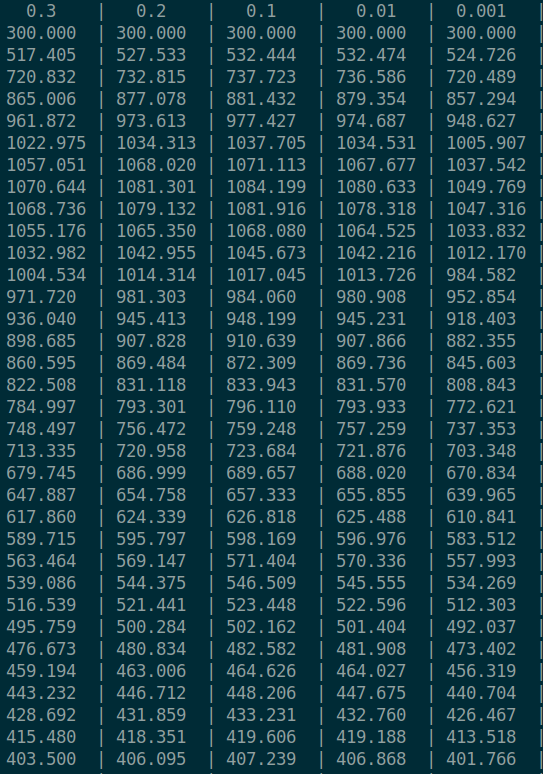
\includegraphics[width=12cm]{tau1tmax140}}
	\caption{$t_{max} = 140, \tau = 1$.}
	\label{fig:1401}
\end{figure}
\newpage
\begin{figure}[!h]
	\center{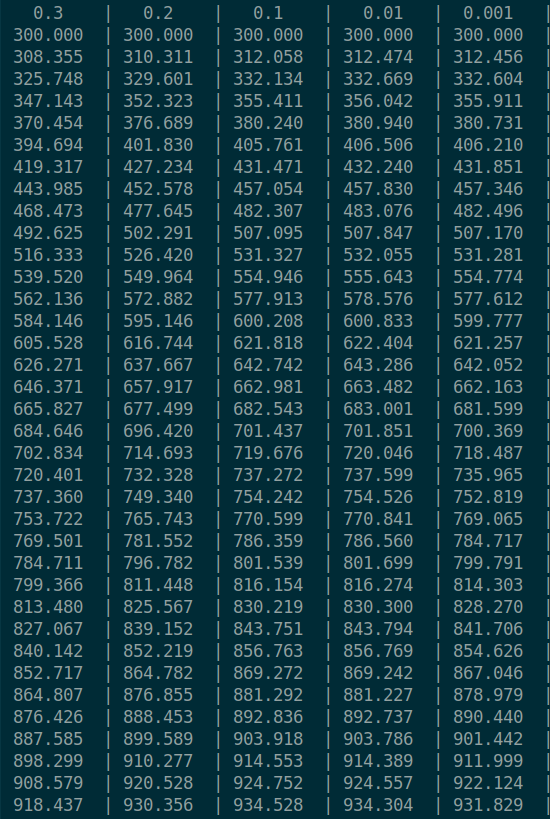
\includegraphics[width=12cm]{tau01tmax140}}
	\caption{$t_{max} = 140, \tau = 0.1$.}
	\label{fig:14001}
\end{figure}
\newpage
\begin{figure}[!h]
	\center{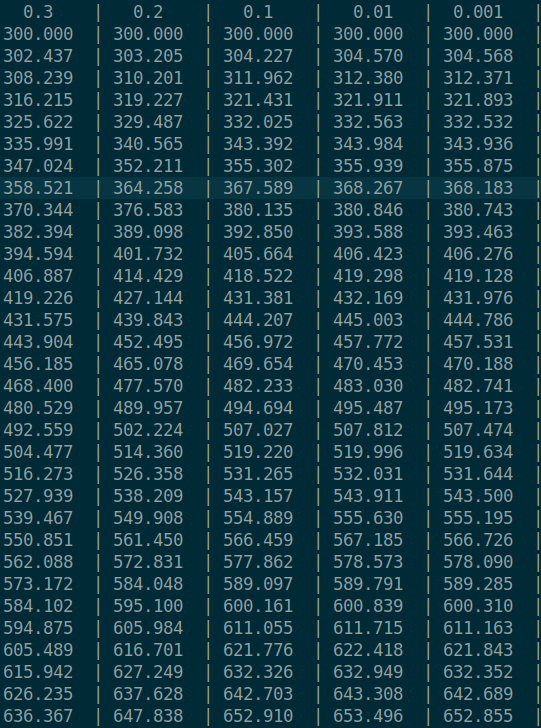
\includegraphics[width=12cm]{tau005tmax140}}
	\caption{$t_{max} = 140, \tau = 0.05$.}
	\label{fig:140005}
\end{figure}
\newpage
\begin{figure}[!h]
	\center{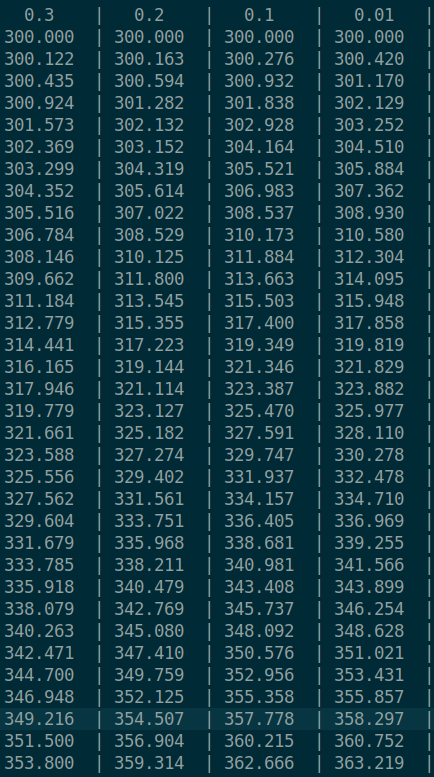
\includegraphics[width=12cm]{tau001tmax140}}
	\caption{$t_{max} = 140, \tau = 0.01$.}
	\label{fig:140001}
\end{figure}

Таким образом, при $t_{max} = 140, F_{max} = 50$, оптимальными
значениями шагов являются $h = 0.01, \tau = 0.1$.

Таким образом, были получены следующие значения оптимальных
шагов (таблица 3).

\begin{table}[!h]
	\caption{Оптимальные шаги.}
	\begin{center}
	\begin{tabular}{| c | c | c |}
	\hline
	$t_{max}$ & $h$ & $\tau$ \\
	\hline
	20 & 0.01 & 0.01 \\
	60 & 0.01 & 0.01 \\
	100 & 0.01 & 0.1 \\
	140 & 0.01 & 0.1 \\
	\hline
	\end{tabular}
	\end{center}
\end{table}

$\tau \approx \frac{t_{max}}{1000}$.

Рассмотрим влияние на получаемые результаты
амплитуды импульса $t_{max}$ и времени $F_{max}$.

Рассмотрим график функции $F(t)$ при $F_{max} = 50, t_{max} = 20$ (рисунок \ref{fig:basegraph}).

\begin{figure}[!h]
	\center{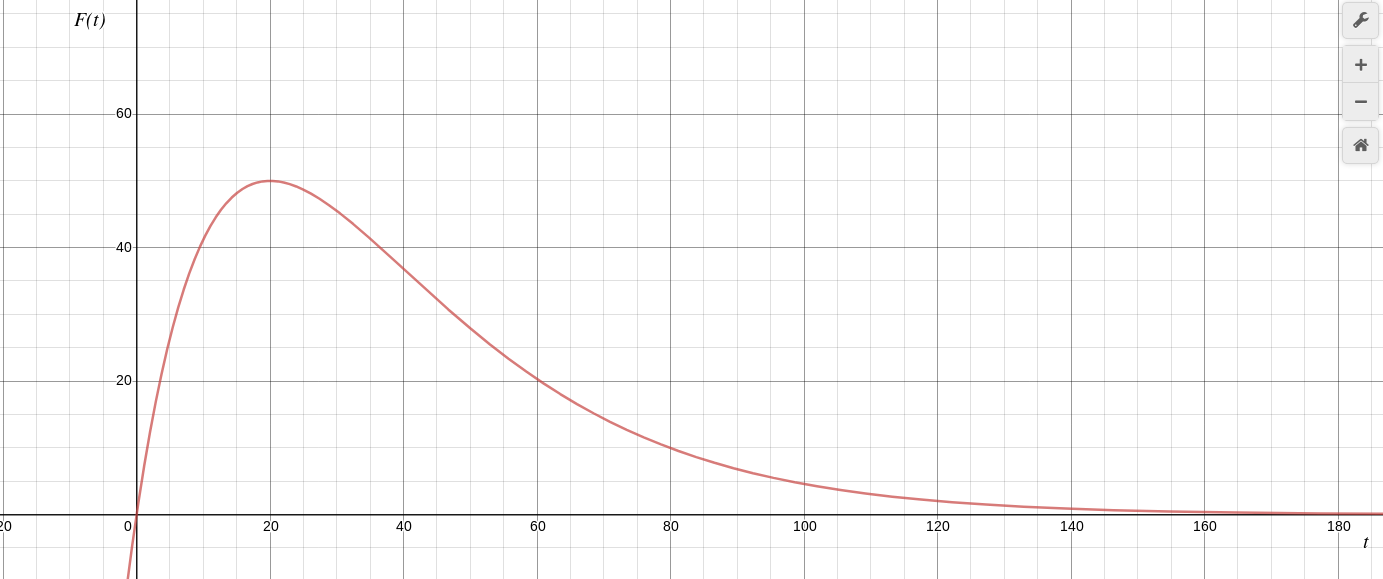
\includegraphics[width=17cm]{Ft}}
	\caption{График функции $F(t)$.}
	\label{fig:basegraph}
\end{figure}

При уменьшении $F_{max}$ график $F(t)$ выглядит так, как на рисунке \ref{fig:lessF},
а при уменьшении $t_{max}$ -- так, как на рисунке \ref{fig:lesst}.

\begin{figure}[!h]
	\center{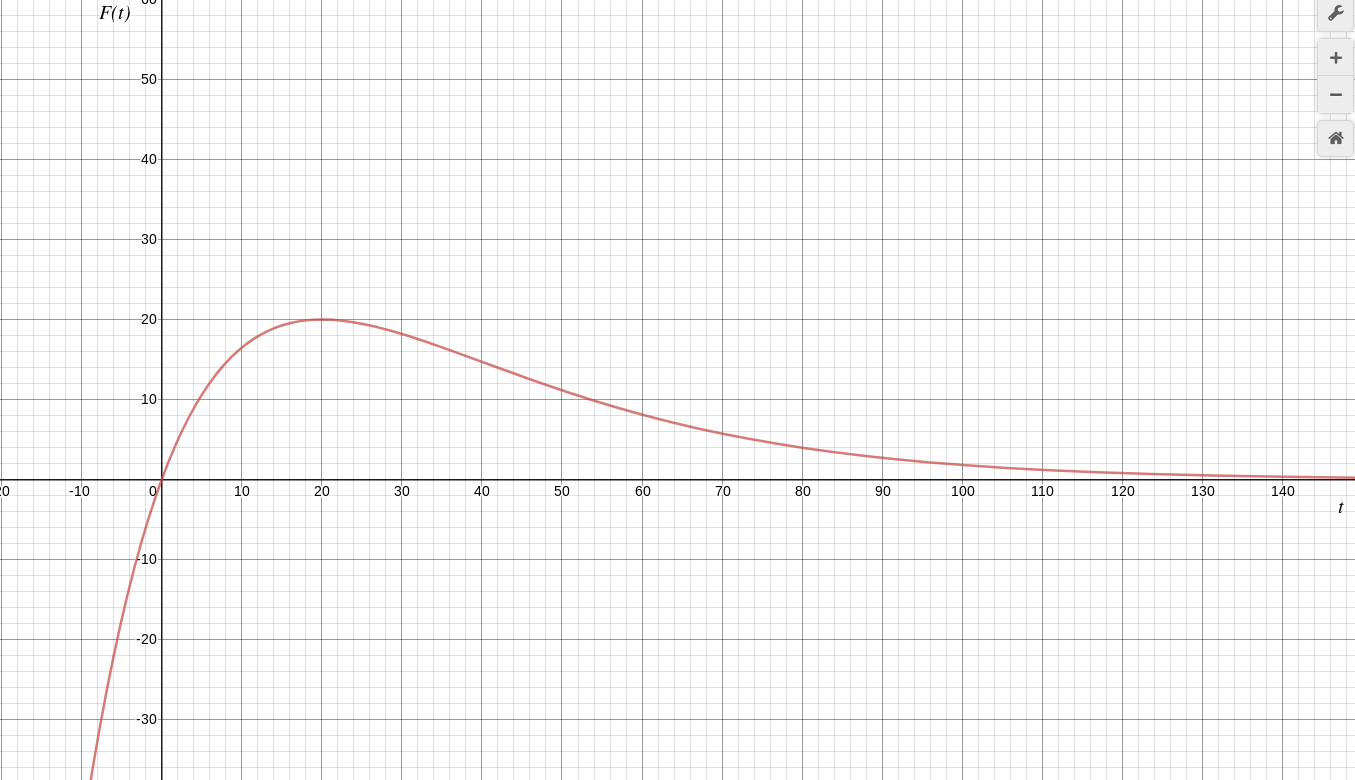
\includegraphics[width=17cm]{lessF}}
	\caption{График функции $F(t)$.}
	\label{fig:lessF}
\end{figure}

\begin{figure}[!h]
	\center{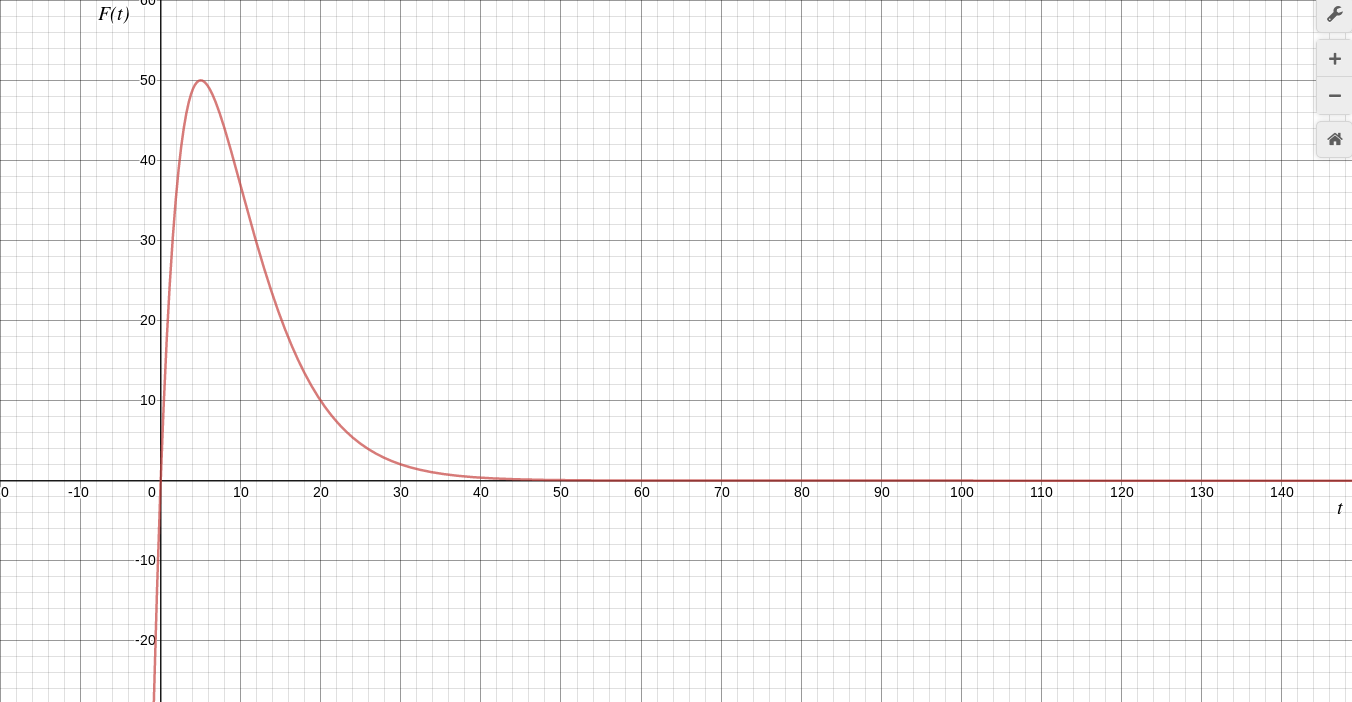
\includegraphics[width=17cm]{lesst}}
	\caption{График функции $F(t)$.}
	\label{fig:lesst}
\end{figure}
\newpage

На рисунках \ref{fig:t10fmax} - \ref{fig:t75fmax}
представлены результаты работы программы при различных значениях
$F_{max}$ и $t_{max}$.

\newpage
\begin{figure}[!h]
	\center{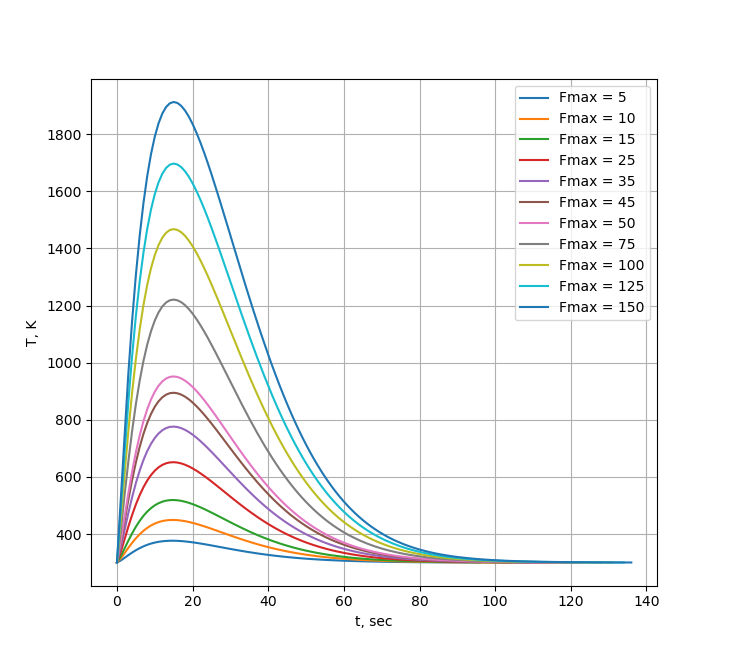
\includegraphics[width=16cm]{t10fmax}}
	\caption{$t_{max}=10$.}
	\label{fig:t10fmax}
\end{figure}
\newpage
\begin{figure}[!h]
	\center{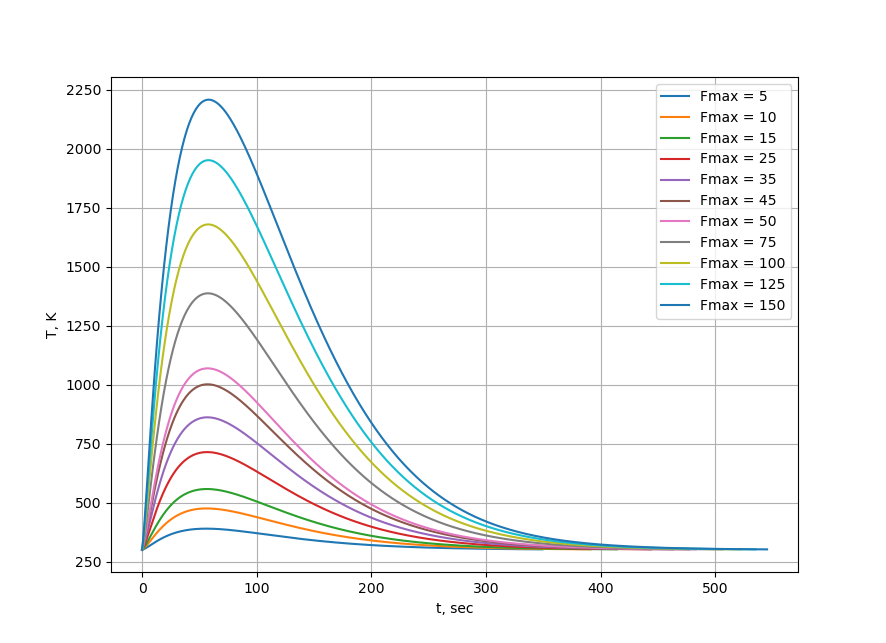
\includegraphics[width=16cm]{t50fmax}}
	\caption{$t_{max}=50$.}
	\label{fig:t50fmax}
\end{figure}
\newpage
\begin{figure}[!h]
	\center{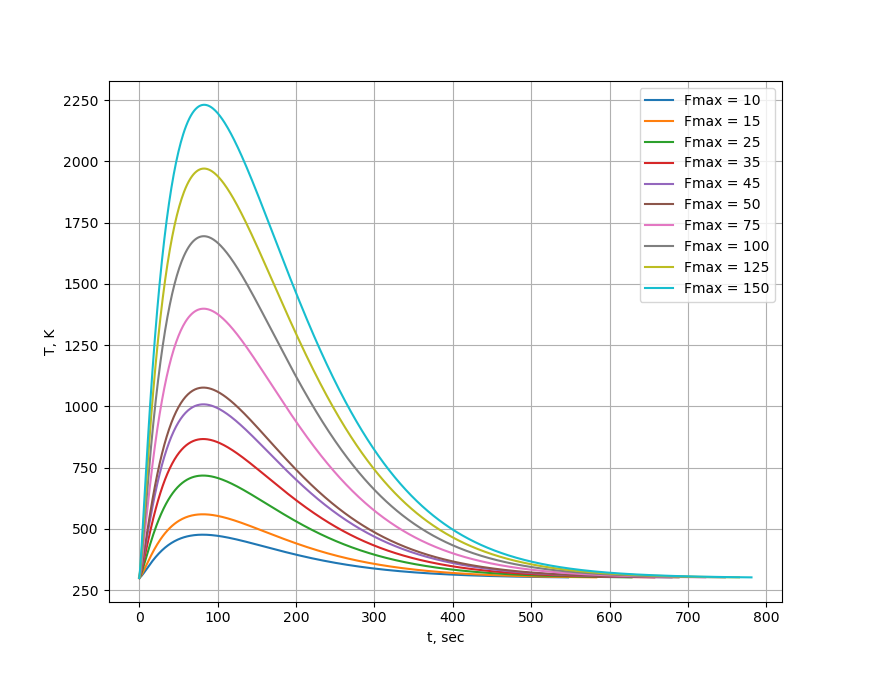
\includegraphics[width=16cm]{t75fmax}}
	\caption{$t_{max}=75$.}
	\label{fig:t75fmax}
\end{figure}

Таким образом, при увеличении $F_{max}$ увеличивается
максимальная температура стержня, а при увеличении
$t_{max}$ меняется время, за которое достигается 
максимальная температура.

\subsubsection*{Задание 2}

График зависимости температуры $T(0, t)$ при различных значениях $a_2$
представлен на рисунке \ref{fig:as}. Измерения проводились с параметрами
$F_{max} = 100, t_{max} = 10, h = 0.01, \tau = 1$.

\newpage
\begin{figure}[!h]
	\center{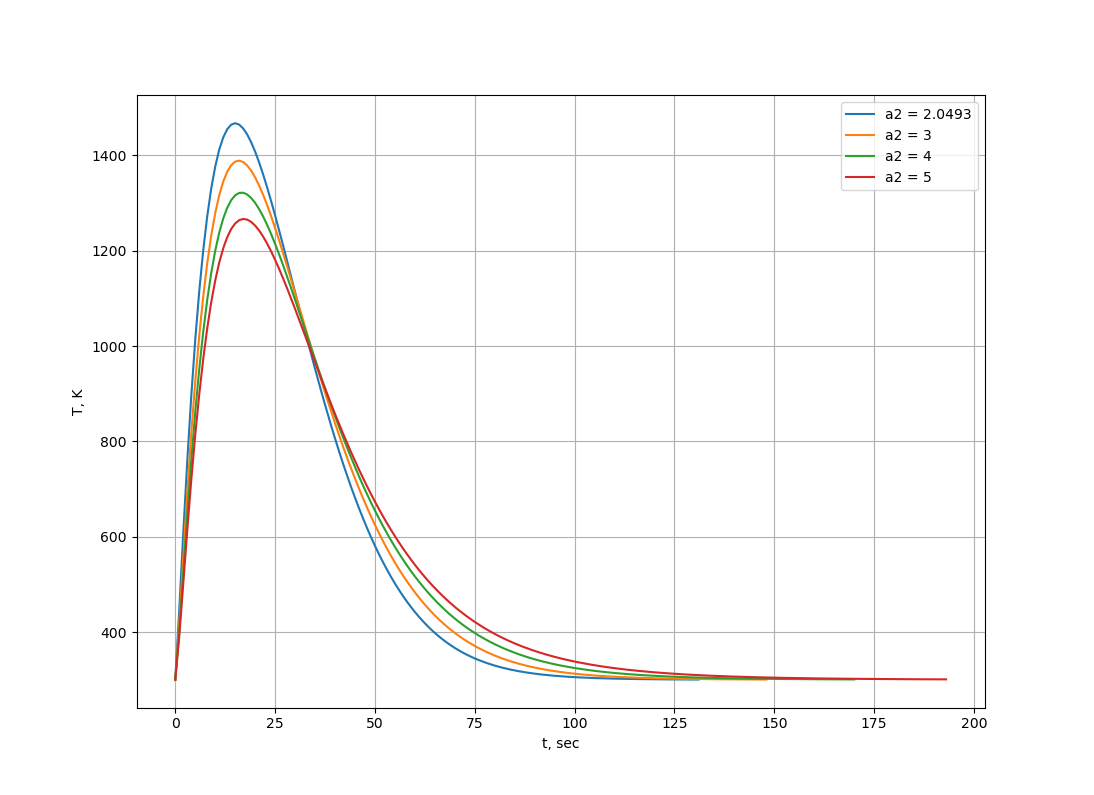
\includegraphics[width=15cm]{Figure_1}}
	\caption{График зависимости температуры $T(0, t)$ при различных значениях $a_2$.}
	\label{fig:as}
\end{figure}


\subsubsection*{Задание 3}

Будем проводить измерения при $F_{max} = 10, t_{max} = 1, h = 0.01, \tau = 0.01$.

Рассмотрим график $F(t)$ на рисунке \ref{fig:al} с $t_{max} = 1, F_{max} = 10$.
Чтобы импульсы при таких параметрах не перекрывались, частота $\nu$
должна быть примерно $\frac{1}{\nu} > 10$, то есть $\nu < \frac{1}{10} = 0.1$.

\begin{figure}[!h]
	\center{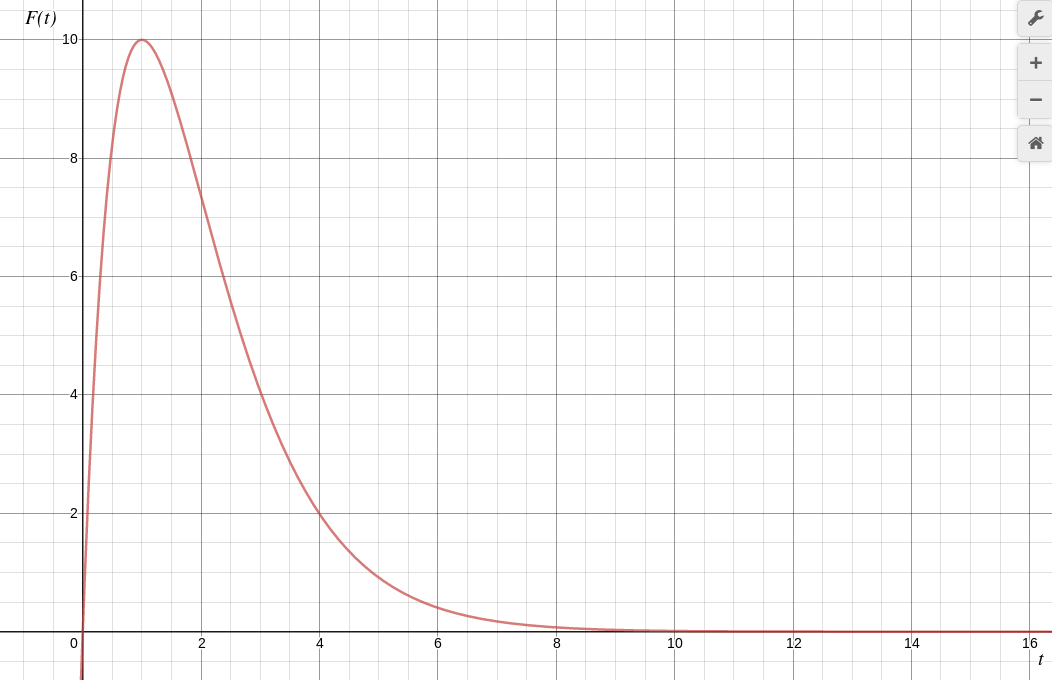
\includegraphics[width=15cm]{al}}
	\caption{$t_{max} = 1, F_{max} = 10$.}
	\label{fig:al}
\end{figure}

На рисунках \ref{fig:start} - \ref{fig:end} изображены результаты работы программы
при различных значениях $\nu$.

\newpage
\begin{figure}[!h]
	\center{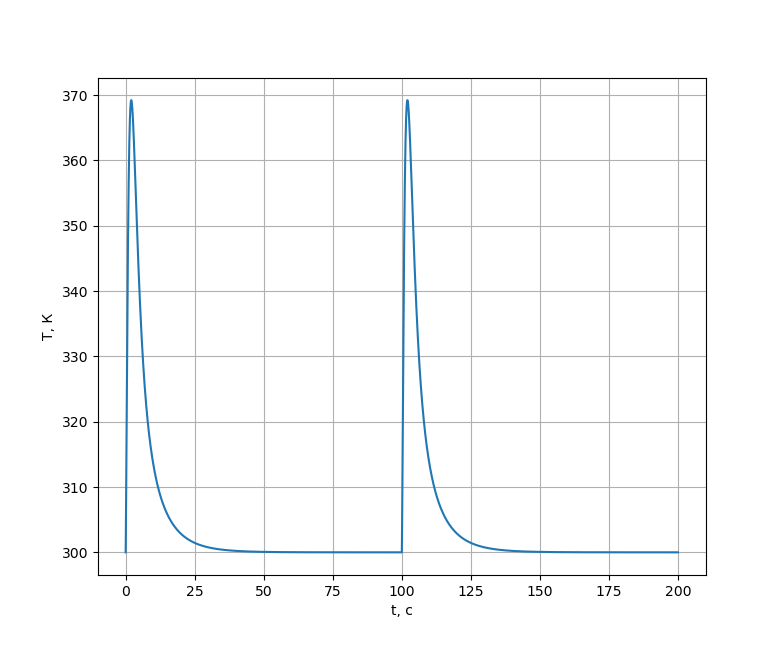
\includegraphics[width=15cm]{Figure_2}}
	\caption{$\nu = 0.01$}
	\label{fig:start}
\end{figure}
\newpage
\begin{figure}[!h]
	\center{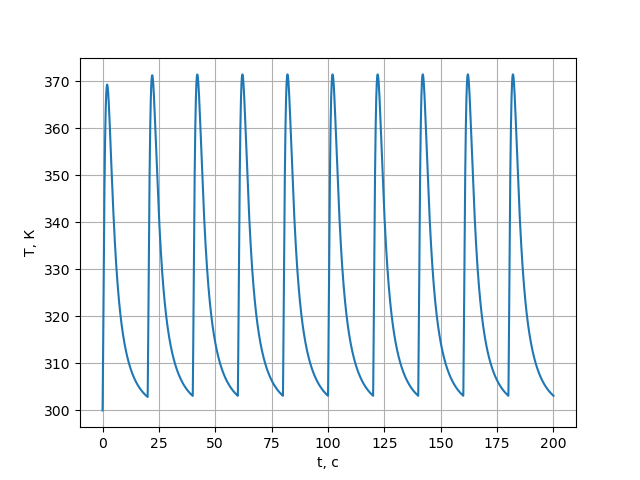
\includegraphics[width=15cm]{Figure_3}}
	\caption{$\nu = 0.05$}
	\label{fig:c1}
\end{figure}
\newpage
\begin{figure}[!h]
	\center{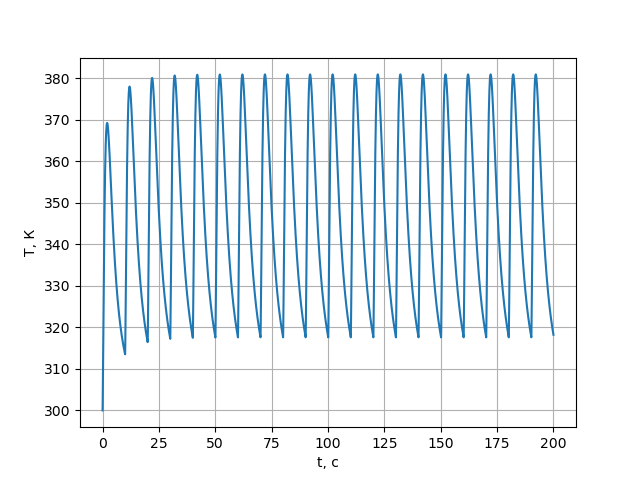
\includegraphics[width=15cm]{Figure_4}}
	\caption{$\nu = 0.1$}
	\label{fig:end}
\end{figure}
%\newpage
%\begin{figure}[!h]
%	\center{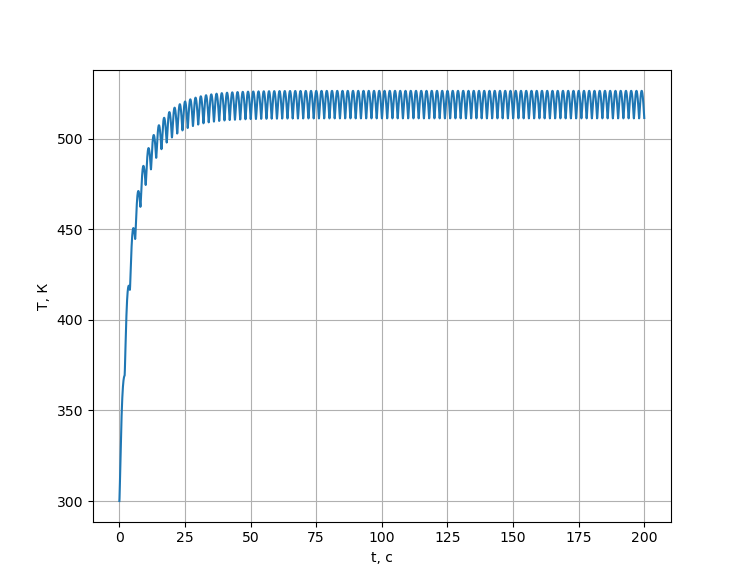
\includegraphics[width=15cm]{Figure_5}}
%	\caption{$\nu = 0.5$}
%	\label{fig:c2}
%\end{figure}
%\newpage
%\begin{figure}[!h]
%	\center{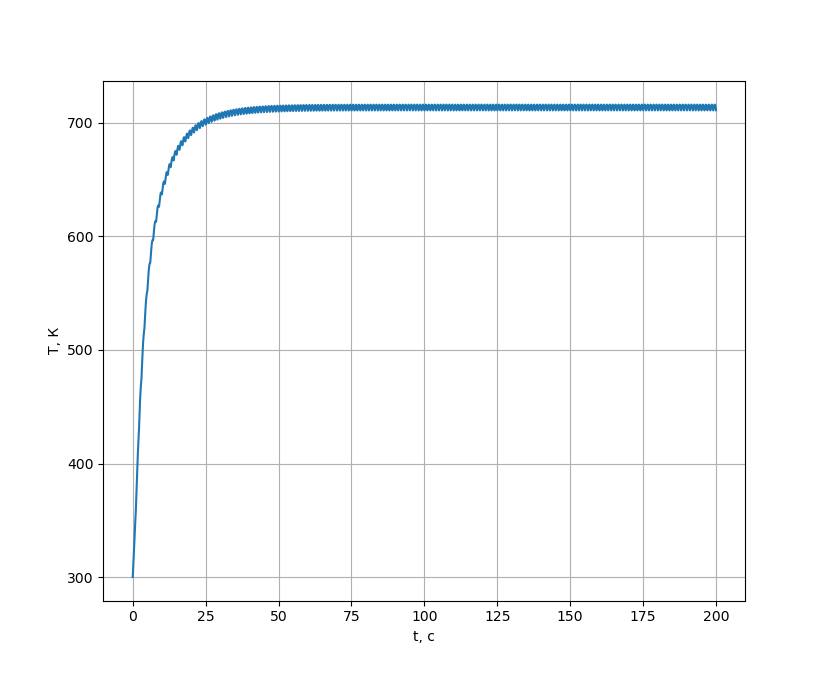
\includegraphics[width=15cm]{Figure_6}}
%	\caption{$\nu = 1$}
%	\label{fig:end}
%\end{figure}
%\newpage
%\begin{figure}[!h]
%	\center{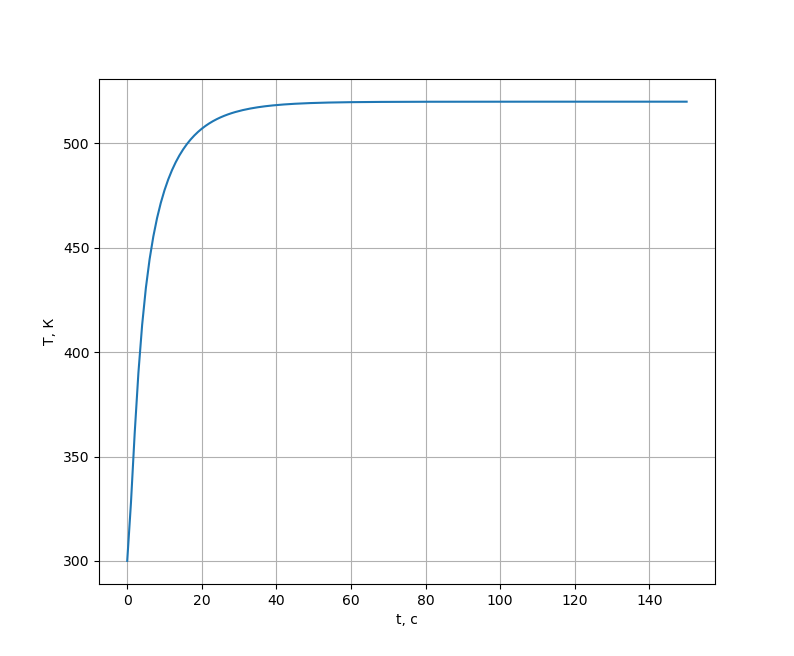
\includegraphics[width=15cm]{compare}}
%	\caption{$\nu = 1$}
%	\label{fig:end}
%\end{figure}

По мере роста частоты импульсов размах колебаний
температуры уменьшается. При этом
реализуется квазистационарный режим, при котором 
в торец поступает постоянный поток $F_c = \nu \int \limits_0^{t_u} F(t) dt$.

При $t_u = 5.5$, $\frac{F(t_u)}{F_{max}} \approx 0.05$.
Поэтому $F_c = 0.1 \int \limits_0^{5.5} \frac{10}{1} t e^{-(\frac{t}{1} - 1)} dt \approx 2.646$.

Сравним полученный результат с результатом расчета $T(x)$ по программе лаб. работы 3 при $F_0=F_c$
и при всех одинаковых параметрах модели, 
в частности, вместо $k(T)$ будем использовать $k(x)$ из лаб. работы 3 
(рисунок \ref{fig:good}).

\newpage
\begin{figure}[!h]
	\center{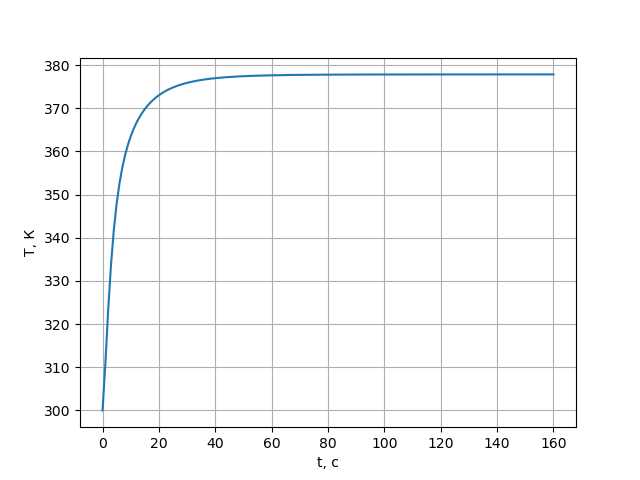
\includegraphics[width=15cm]{good}}
	\caption{График из лабораторной работы 3.}
	\label{fig:good}
\end{figure}


\subsection*{Вывод}

Таким образом, в ходе данной работы были получены навыки 
проведения исследований компьютерной математической модели,
построенной на квазилинейном уравнении параболического типа.

\end{document}

\end{document}